\documentclass[dvipsnames]{beamer}

\usepackage[utf8]{inputenc}
\usetheme{default}
\usefonttheme[onlymath]{serif}
\useinnertheme{circles}

%% set colours
\definecolor{atugreen}{HTML}{005b5e}
\setbeamercolor{title}{fg=atugreen}
\setbeamercolor{frametitle}{fg=atugreen}
\setbeamercolor{section in toc}{fg=atugreen}
\setbeamercolor{itemize item}{fg=atugreen}
\setbeamercolor{itemize subitem}{fg=orange}
\setbeamertemplate{section in toc}{\inserttocsectionnumber.~\inserttocsection}
\setbeamercolor{section number projected}{bg=white,fg=atugreen}

\title{ GLM fundamentals\\ A gentle theory of the three pillars of\\response, link and linear predictor
}
\author{Cóilín Minto, Olga Lyashevska}
\date{July 15\textsuperscript{th} 2022}
\institute{Marine and Freshwater Research Centre\\ Atlantic Technological University \\ Galway, Ireland}
%% logo
\titlegraphic{
    
\includegraphics[width=4cm]{figures/ATU-Logo-Full-RGB-Green-big.jpg}
}

\AtBeginSection[]{
\begin{frame}[noframenumbering, plain]
\frametitle{Outline}
\tableofcontents[currentsection]
\addtocounter{page}{-1}
\end{frame}
}

\begin{document}

\begin{frame}
 \maketitle
\end{frame}
\section{A little history}
\begin{frame}
 \frametitle{A little bit about GLMs}
 Developed by Nelder and Wedderburn (1972)\footnote{\tiny Nelder, J. and Wedderburn, R. (1972). Generalized Linear Models. \emph{Journal of the Royal Statistical Society. Series A (General)}, 135 (3), 370--384.}
 %%
 \begin{center}
    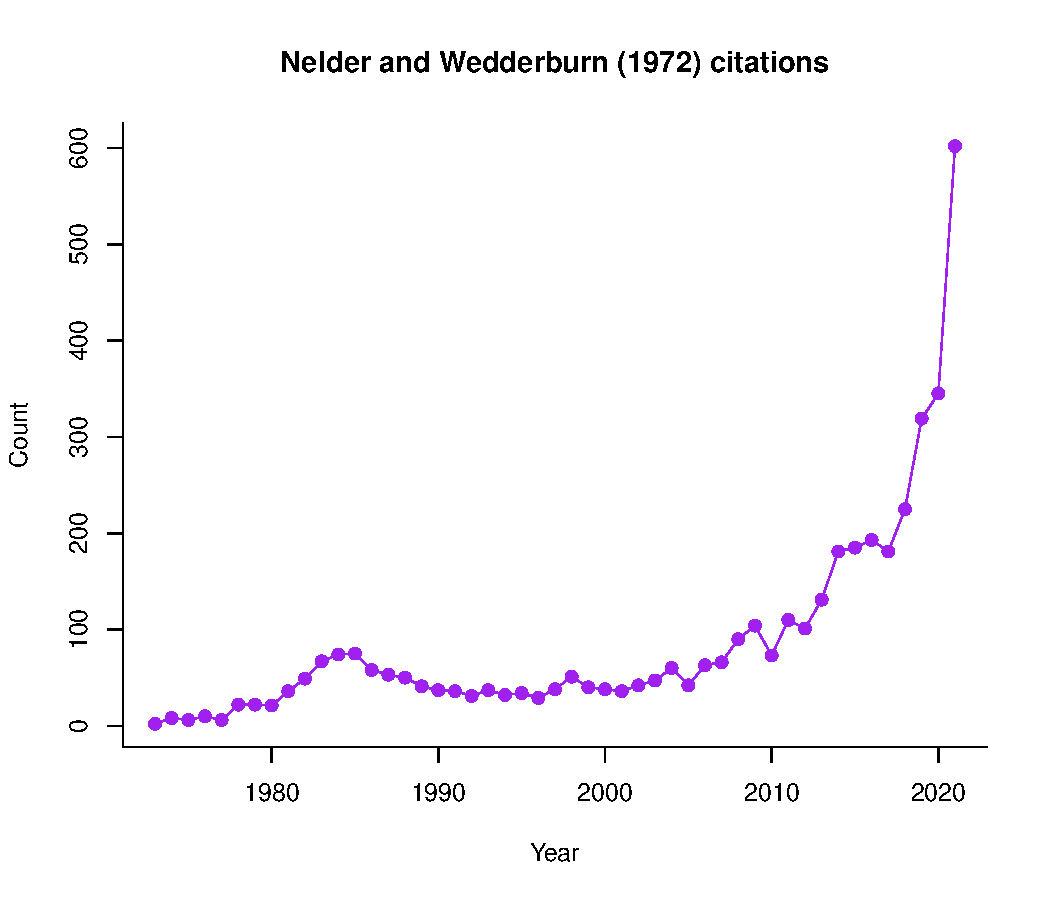
\includegraphics[width=8cm]{figures/glm_citations.pdf}
 \end{center}
\end{frame}

\begin{frame}
 \frametitle{A little bit about GLMs}
Famous book - McCullagh and Nelder (cited $>$43,000 times)
 \begin{center}
    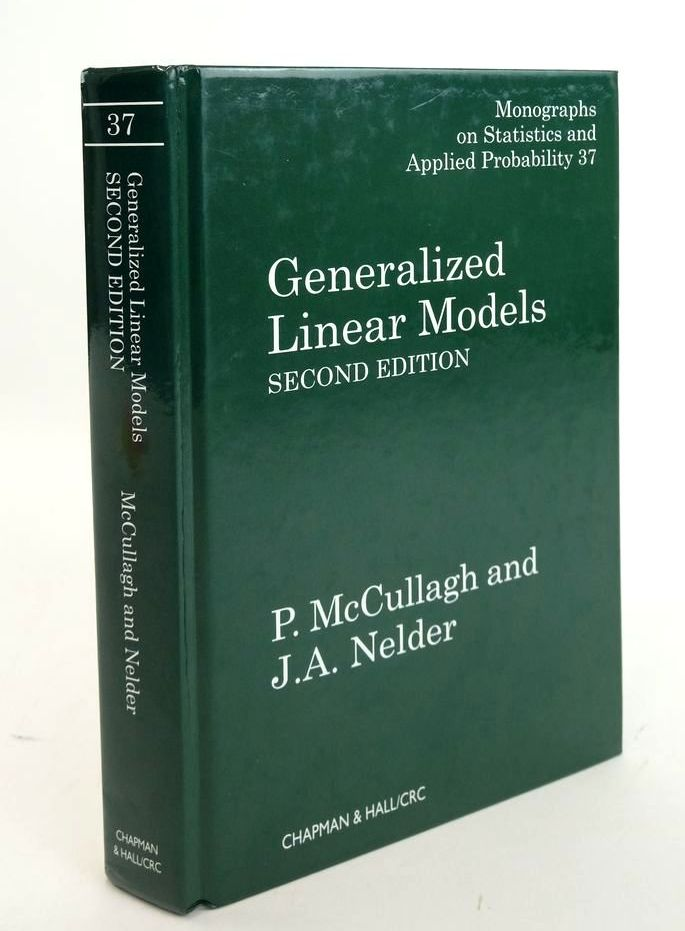
\includegraphics[width=5cm]{figures/glm_book.jpeg}
 \end{center}
\end{frame}

\section{GLM components}
\begin{frame}
 \frametitle{Linear regression - normal errors}
\begin{center}
  \includegraphics<1-1>[width=10cm]{figures/continuous_y_0.pdf}
  \includegraphics<2-2>[width=10cm]{figures/continuous_xy_0.pdf}
\end{center}
\end{frame}

\begin{frame}
 \frametitle{Linear regression - normal errors}
For the linear regression
\begin{equation*}
 y \sim \textrm{N}(\mu,\sigma^2)
\end{equation*}
where 
\begin{equation*}
 \mu = a+bx
\end{equation*}
what are $a$ and $b$?
\end{frame}

\begin{frame}
 \frametitle{Nonnormal errors}
Often errors are non-normally distributed:
\begin{itemize}
 \item May exhibit a lot of skew
 \item Exhibit heavy tails
 \item Discrete variable (e.g. count, especially low counts)
 \item May be bounded (e.g. binary data)
\end{itemize}
In these cases, the use of normal distribution is typically not appropriate 
\end{frame}

\begin{frame}
 \frametitle{Nonnormal errors}
Traditional approach has been to transform the data prior to analysis to achieve:
\begin{itemize}
 \item Constancy of the variance (normality)
 \item Additivity of effects $bx+cz$
\end{itemize}
Transformations sometimes work spectacularly well (lognormal data), where log transforming stabilizes the variance and results in additivity but for other data (counts) most transforms cannot achieve both goals
\end{frame}

\begin{frame}
 \frametitle{Generalized Linear Models (GLMs)}
GLMs allow one to fit normal and non-normal error models from the exponential family, including:
\begin{itemize}
 \item Binomial
 \item Poisson
 \item Gamma
 \item Normal
 \item \dots
\end{itemize}

\end{frame}

\begin{frame}
 \frametitle{Three components of a GLM}
 \begin{center}
\begin{tabular}{ll}
Distribution & \begin{minipage}[c][2cm][c]{.2\textwidth}  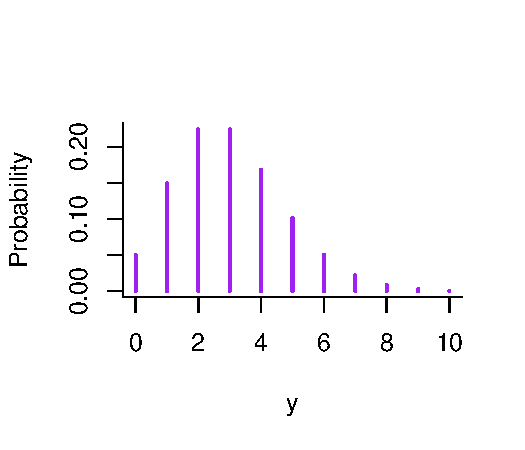
\includegraphics[width=4cm]{figures/distribution.pdf}\end{minipage}\\
Link function & \begin{minipage}[c][2cm][c]{.2\textwidth}  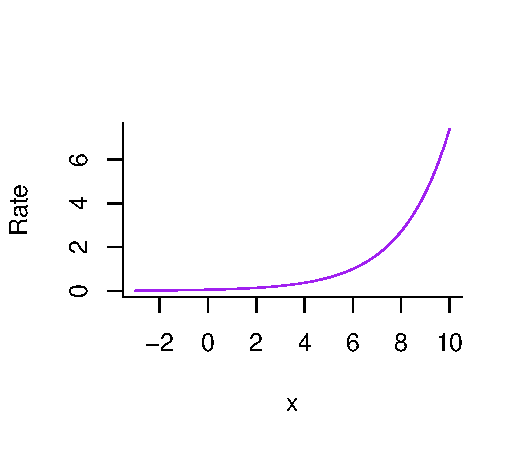
\includegraphics[width=4cm]{figures/link_function.pdf}\end{minipage}\\
Linear predictor & \begin{minipage}[c][4cm][c]{.2\textwidth}  
\includegraphics[width=3cm]{figures/Science-symbol-2.svg.png}\end{minipage}
 \end{tabular}
 \end{center}
\tiny{\url{https://commons.wikimedia.org/wiki/File:Science-symbol-2.svg}}
\end{frame}

\begin{frame}
 \frametitle{Distribution}
 \begin{center}
    \includegraphics<1-1>[width=10cm]{figures/normal_0.pdf}
    \includegraphics<2-2>[width=10cm]{figures/lognormal_0.pdf}
    \includegraphics<3-3>[width=10cm]{figures/poisson_0.pdf}
    \includegraphics<4-4>[width=10cm]{figures/binomial_0.pdf}
 \end{center}
\end{frame}

\begin{frame}
 \frametitle{Link function}
 Link function transforms parameter from its natural scale (positive, between zero and one, \dots) to the real line.\\ 
 Think of it as a way to make sure the parameter is bounded correctly
\end{frame}

\begin{frame}
 \frametitle{Link function examples}
 \begin{center}
    \onslide<1-1>{Identity\\}
    \onslide<2-2>{Log\\} \vspace{-1cm}
    \onslide<3-3>{Logit\\} \vspace{-1cm}
    \includegraphics<1-1>[width=9cm]{figures/identity_link.pdf}
    \includegraphics<2-2>[width=9cm]{figures/log_link.pdf}
    \includegraphics<3-3>[width=9cm]{figures/logit_link.pdf}
 \end{center}
\end{frame}

\begin{frame}
 \frametitle{Linear predictor}
 \begin{center}
 Where the science (aka hypotheses) enters!
 
\includegraphics[width=6cm]{figures/Science-symbol-2.svg.png}
 \end{center}
\tiny{\url{https://commons.wikimedia.org/wiki/File:Science-symbol-2.svg}}
\end{frame}

\begin{frame}
 \frametitle{Linear predictor}
Example - for a whale survey we might be interested in whether the sighting rate depends on water surface temperature
\begin{equation*}
 \log(\lambda) = a + b * SST
\end{equation*}
our inference concerns whether $b=0$ or not
\end{frame}

\begin{frame}[fragile]
 \frametitle{Poisson GLM}
%\begin{eqnarray*}
% Distribution & y&\sim& \textrm{Pois}(\lambda)\\
% Link function& \ln(\lambda)&=& \eta\\
% Linear predictor & \eta&=&a+b* SST \\
%\end{eqnarray*}
\begin{center}
\begin{tabular}{lr}
Distribution: & $y \sim \textrm{Pois}(\lambda)$\\
&\\
Link function: & $\log(\lambda) = \eta$ \\
&\\
Linear predictor: & $\eta = a+b* SST$
\end{tabular}
\end{center}
NB: $a$ and $b$ are what \texttt{glm} in R will estimate and report 
\end{frame}

\begin{frame}[fragile]
 \frametitle{Link function: binomial}
The default link function relating the mean and the linear predictor for Binomial is the logit
\begin{equation*}
 \textrm{logit}(p)=\eta
\end{equation*}
where $\eta$ is the linear predictor (where your covariates enter)\\
\begin{equation*}
\textrm{logit}(p)=\ln\left(\frac{p}{1-p}\right)
\end{equation*}
\end{frame}

\begin{frame}
 \frametitle{Linear predictor: binomial}
Example - interested in how maturity changes over length of fish
\begin{equation*}
\textrm{logit}(p)=a + b * length
\end{equation*}
\end{frame}

\begin{frame}
\frametitle{Binomial GLM}
\begin{center}
\begin{tabular}{lr}
Distribution: & $y \sim \textrm{Bin}(n,p)$\\
&\\
Link function: & $\textrm{logit}(p) = \eta$ \\
&\\
Linear predictor: & $\eta = a+b*length$
\end{tabular}
\end{center}
NB: $a$ and $b$ are what \texttt{glm} in R will estimate and report 
\end{frame}

\section{Predictions via inverse link functions}

\begin{frame}
 \frametitle{Inverse link function}
 \begin{center}
\begin{tabular}{lll}
Distribution & Link function & Inverse link\\
\hline
Poisson & $\log$ & $\exp$\\
Binomial & $\textrm{logit}$  & $\textrm{logit}^{-1}$ (\texttt{plogis} in R)
 \end{tabular}
 \end{center}
 
 Use the inverse link to get predictions on the scale of the data (will see more on this in the practicals)
\begin{center}
        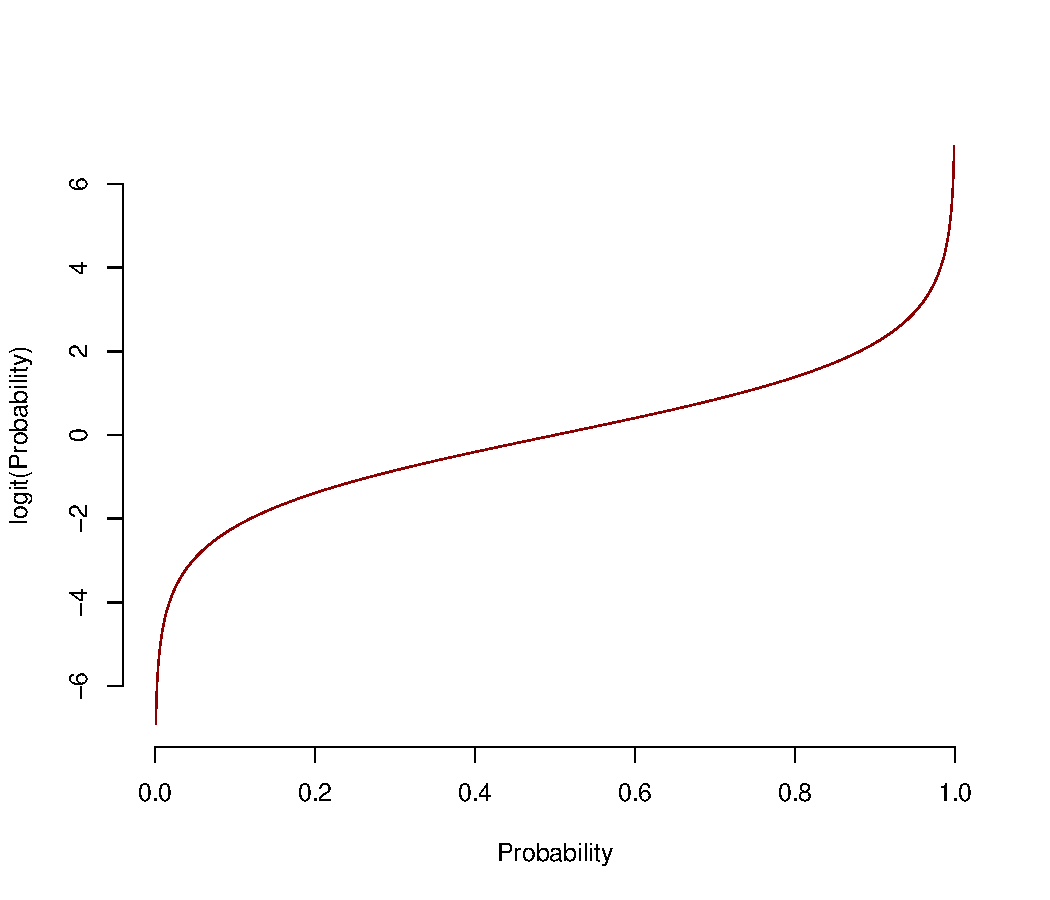
\includegraphics[width=0.6\textwidth]{figures/logit_link.pdf}
\end{center}
\end{frame}

\section{Summary}
\begin{frame}
 \frametitle{Summary}
  \begin{itemize}
  \item<1-> GLMs used very widely
  \item<2-> GLMs allow for natural distributions matching the data type
  \item<3-> Three components: 
    \begin{itemize}
    \item Distribution
    \item Link function
    \item Linear predictor
     \end{itemize}
 \end{itemize}
\end{frame}


\begin{frame}
\begin{center}
Questions? 
\end{center}
\end{frame}
 


\end{document}

\begin{frame}
 \frametitle{}
\end{frame}
